\documentclass[11pt,a4paper]{article}

\usepackage[utf8]{inputenc}
\usepackage[T1]{fontenc}
\usepackage{amsmath, amssymb}
\usepackage{graphicx}
\usepackage{geometry}
\usepackage{hyperref}
\usepackage{booktabs}
\usepackage{float}
\usepackage{siunitx}
\usepackage{xcolor}

\geometry{a4paper, margin=2.5cm}
\newcommand{\HRule}{\rule{\linewidth}{0.5mm}}

\title{PHYS551 Term Project}
\author{Ömer Faruk Avcı}
\date{June 12, 2026}

\begin{document}

% ============================ TITLE PAGE ============================
\begin{titlepage}
\begin{center}


\includegraphics[width=0.50\textwidth]{ozu.png}~\\[2.2cm]

{\Large \textbf{PHYS 551 -- Advanced Monte Carlo Methods}}\\[0.6cm]
{\large Spring 2025/26}\\[0.6cm]
{\large \textbf{TERM PROJECT}}\\[0.8cm]

\HRule \\[0.5cm]
{\LARGE \textbf{Rare-Event Estimation of Cascading Blackouts in the Istanbul
Power Grid via Importance Sampling}}\\[0.5cm]
\HRule \\[2.5cm]

{\large
\textbf{Submitted by:} Ömer Faruk Avcı\\[0.2cm]
\textbf{Student ID:} S034113\\[0.2cm]
\textbf{Course Instructor:} Prof.\ Taylan Akdoğan\\[0.2cm]
\textbf{Date of Submission:} \today
}

\vfill
\textsc{\large Department of Electrical and Electronics Engineering}

\end{center}
\end{titlepage}

% ============================ INTRODUCTION ============================
\section{Introduction}

A large electrical grid does not fail one component at a time. When a single
district is pushed past the limit of its substations, its excess load does not
simply vanish; it is rerouted onto the neighbouring districts. If those
neighbours are themselves close to their limit, the overload spreads, and a
local fault grows into a city-wide blackout. This chain reaction is called a
\emph{cascading failure}. Because the number of possible failure combinations in
a grid of tens of districts is enormous, and because the truly catastrophic
events are very rare, deterministic worst-case analysis is not practical. This
term project therefore studies the problem with Monte Carlo simulation.

The grid studied here is the mainland of Istanbul, modelled as 38 districts on
the European and Asian sides. Each district has a population, a daily
electricity load, and a safety margin that is calibrated from real overload
records published by EPİAŞ. The central difficulty is that a blackout affecting
millions of people is a \emph{rare event}: under normal operation it almost never
happens, so a naive (crude) Monte Carlo simulation would have to run for an
impractically long time before it ever observed one. The project answers two
questions:

\begin{enumerate}
    \item What is the probability that a cascading failure leaves at least $X$
    people without power on a given day, including the rare tail that naive
    Monte Carlo cannot reach? I answer this with \textbf{Importance Sampling}.
    \item Given the resulting risk map, \emph{where} should new relief
    substations be built to reduce the expected number of people affected the
    most?
\end{enumerate}

The remainder of this report is organised as follows. Section~2 describes the
data and the model: the districts, how loads and safety margins are obtained,
and the cascading-failure mechanism. Section~3 presents the naive Monte Carlo
baseline and shows where it breaks down. Section~4 introduces the Importance
Sampling estimator and the systemic-surge bias that makes the rare tail
tractable. Section~5 compares the two methods directly through the exceedance
curve, the variance-reduction table, and a convergence study. Section~6 applies
the model to the substation-placement question. Section~7 concludes.

\subsection*{Declaration of AI Usage}

In compliance with the course's principles for the responsible use of AI, I
disclose my use of AI tools in this project. The Python code was written by an AI
assistant following my prompts and direction. The core of the work, however, is
my own: the design of the algorithm and how the model works -- the
cascading-failure mechanism, the systemic-surge demand model, and the Importance
Sampling scheme -- together with the calibration choices and the sourcing of the
real data (the EPİAŞ electricity-consumption and overload ``Aşırı Yük'' records
that set the district loads and safety margins) were all done by me. I directed
the AI at each step and reviewed and verified every result against the
simulation before including it.

% ============================ MODEL & DATA ============================
\section{System Model and Data}

\subsection{Districts, Population, and Load}

The grid is represented as a graph of 38 mainland districts (the islands are
excluded), with a total population of about \num{15736564}. Two districts are
connected by an edge if they share a physical border, giving 83 edges; the
adjacency was extracted from district geometry and adjusted for the Bosphorus
bridge crossings. Figure~\ref{fig:graph} shows the resulting network.

Each district is assigned a base electricity load $\mu_i$. The total monthly
consumption of the European and Asian distribution regions (from EPİAŞ
consumption data) is distributed among the districts of each side in proportion
to their population:
\begin{equation}
    \mu_i = C_{\text{side}} \cdot \frac{\text{Pop}_i}{\sum_{j \in \text{side}} \text{Pop}_j},
\end{equation}
where $C_{\text{side}}$ is the average load of the side that district $i$ belongs
to. This makes the load distribution reflect the real demand split between the
two sides of the city.

\begin{figure}[H]
    \centering
    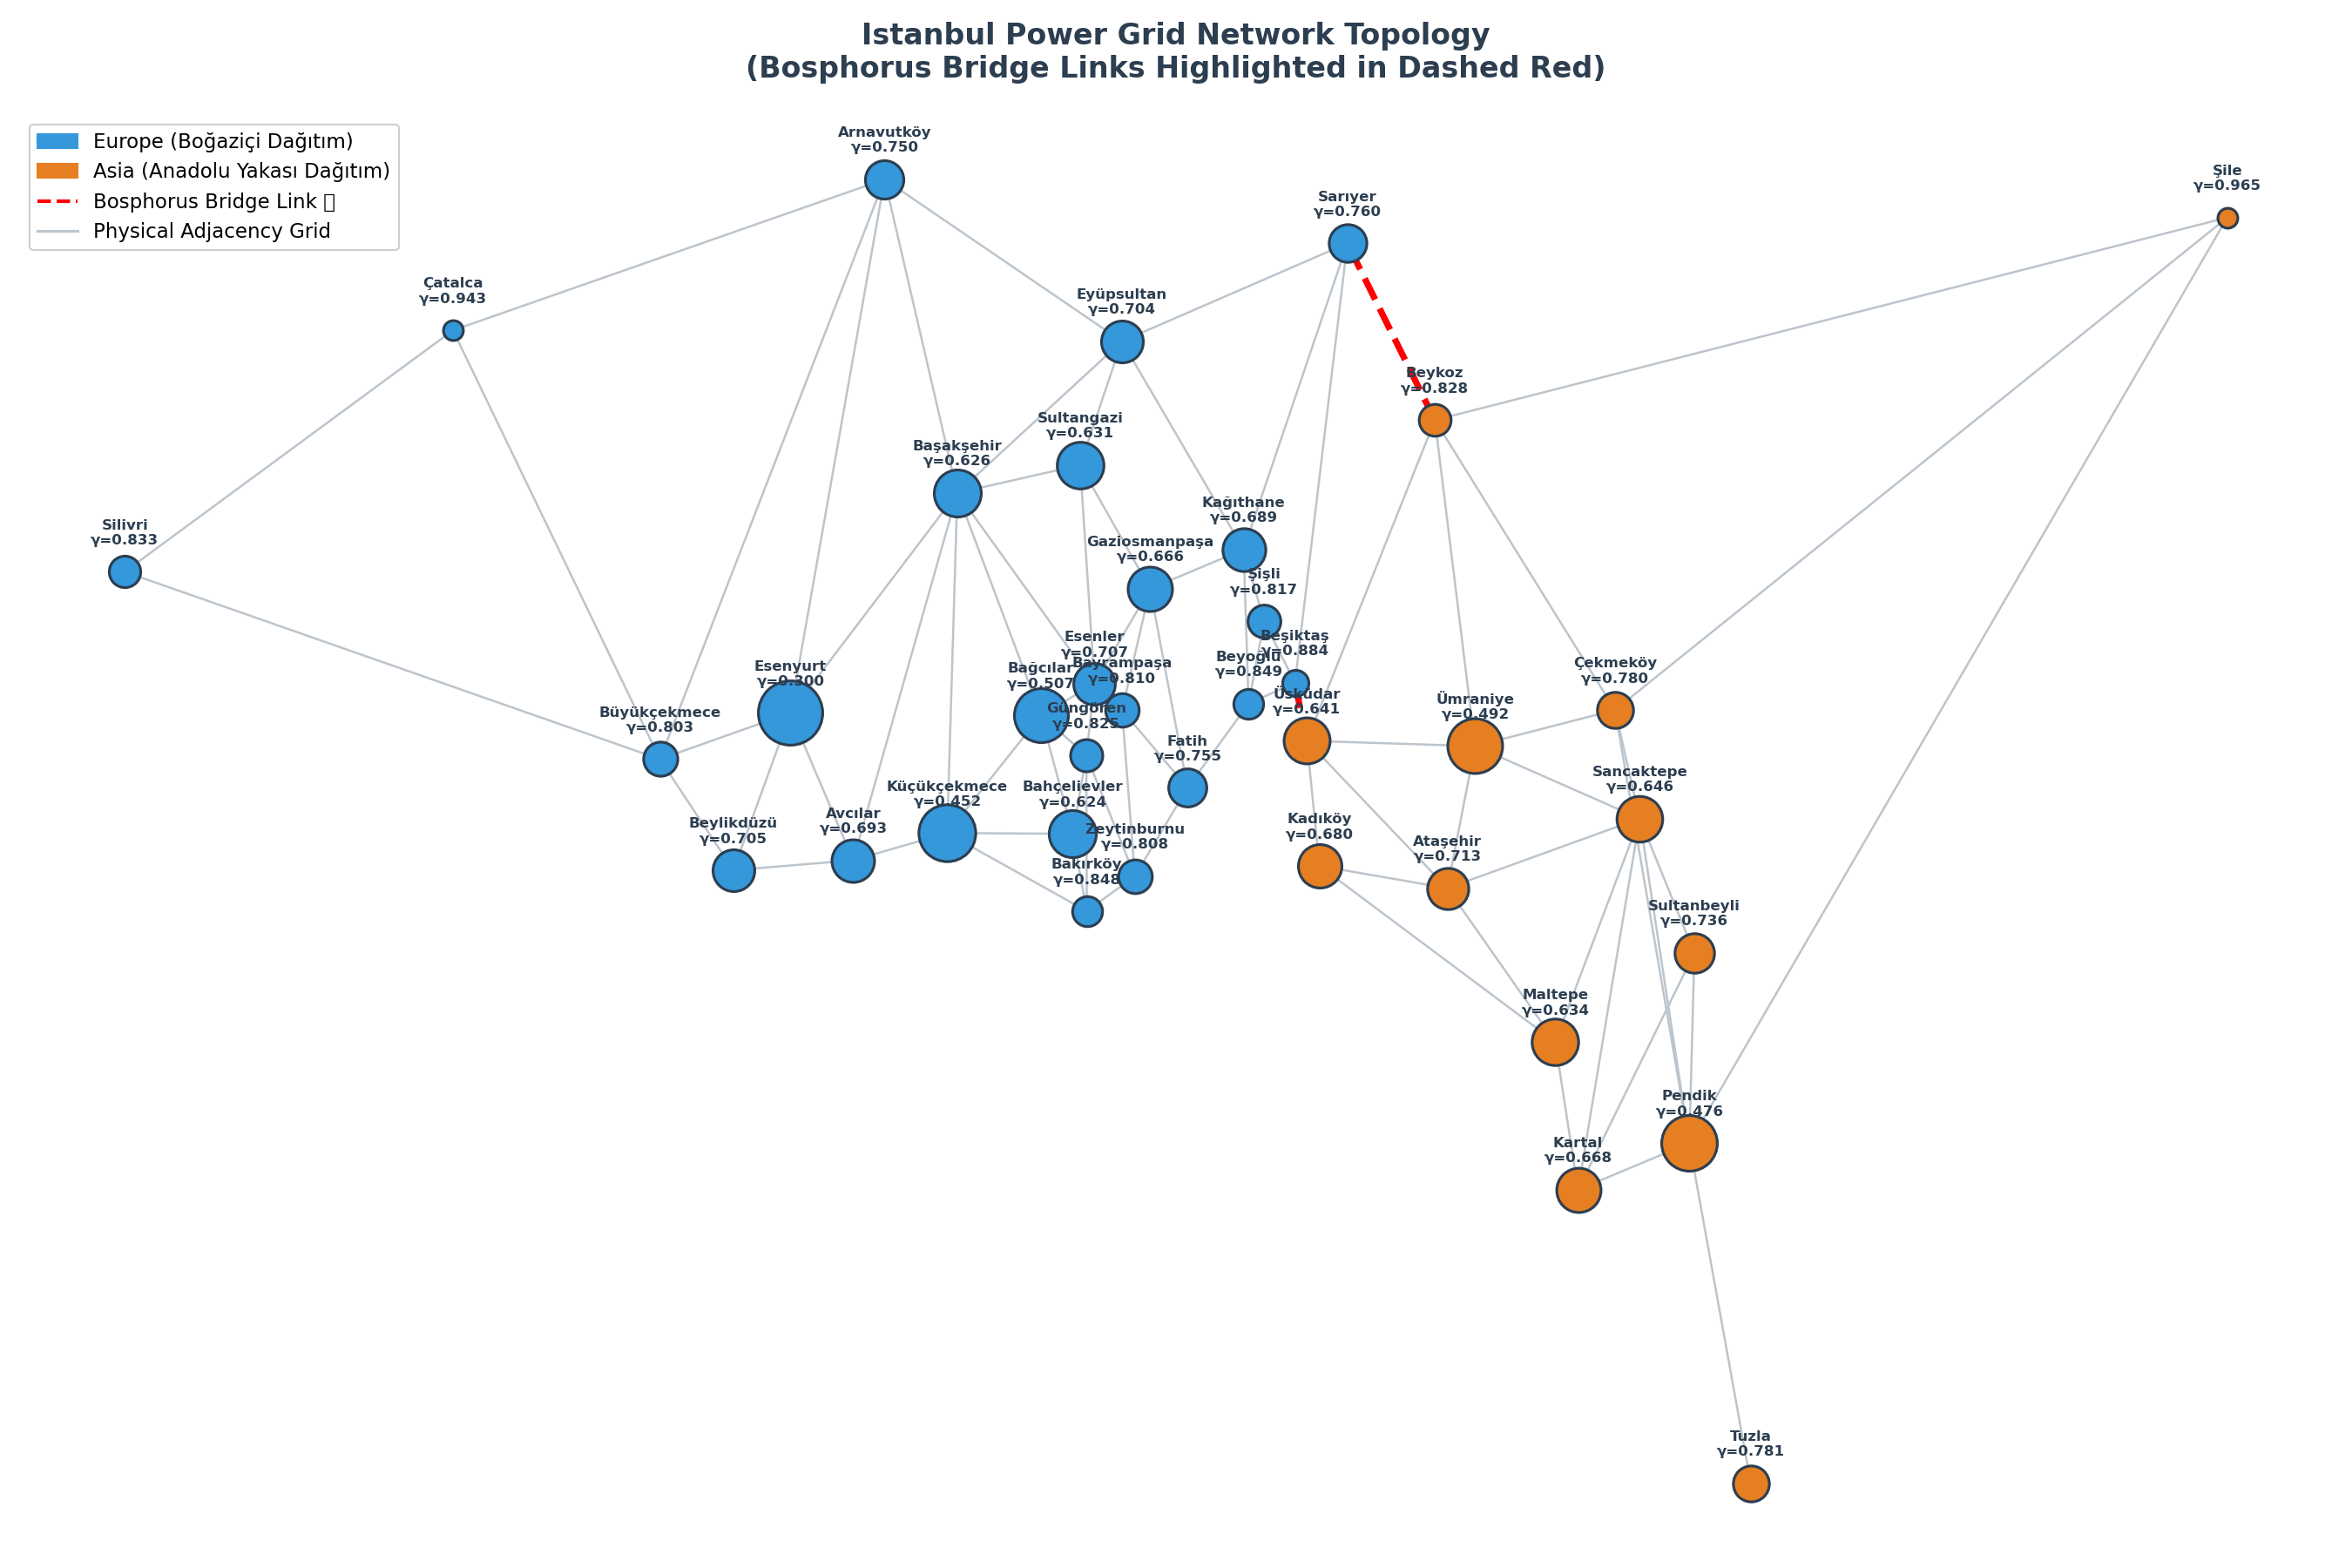
\includegraphics[width=0.92\textwidth]{figures/grid_graph.png}
    \caption{The Istanbul mainland grid as a graph of 38 districts. Nodes are
    placed at district centroids; edges connect bordering districts.}
    \label{fig:graph}
\end{figure}

\subsection{Safety Margins from Real Overload Data}

Each district is given a dimensionless safety margin $\alpha_i$, defined so that
its capacity is
\begin{equation}
    \text{capacity}_i = \mu_i \, (1 + \alpha_i).
\end{equation}
A district with a large $\alpha_i$ can absorb a big demand spike before tripping;
a district with a small $\alpha_i$ is fragile. Rather than assign these margins
arbitrarily, they are calibrated from one year of EPİAŞ outage records by
counting, for each district, how many outages were caused by overload
(``Aşırı Yük''). The margins are then assigned \emph{per side} (because the two
sides are operated by different distribution companies) by linearly mapping the
overload count to the range $[\alpha_{\min}, \alpha_{\max}] = [0.08, 0.25]$:
\begin{equation}
    \alpha_i = \alpha_{\max} - \frac{n_i}{\max_{j \in \text{side}} n_j}\,(\alpha_{\max} - \alpha_{\min}),
\end{equation}
where $n_i$ is the overload count of district $i$. The districts with the most
recorded overloads are therefore given the smallest margins. For example,
Maltepe (465 overloads, the worst on the Asian side) and Fatih and Beyoğlu (108
each, the worst on the European side) receive $\alpha = 0.08$, while a quiet
district such as Çatalca (2 overloads) is close to $\alpha = 0.25$. This is what
makes the model data-driven: the historically weakest districts are the
structurally weakest in the simulation.

\subsection{The Cascading-Failure Mechanism}

\paragraph{Daily demand.}
Electricity demand fluctuates from day to day. The demand of district $i$ on a
given day is modelled as
\begin{equation}
    L_i = \mu_i \, (S + \varepsilon_i),
\end{equation}
where $S \sim \mathcal{N}(1, \sigma_{\text{sys}}^2)$ is a single
\textbf{city-wide demand multiplier} shared by every district, and
$\varepsilon_i \sim \mathcal{N}(0, \sigma_{\text{idio}}^2)$ is a small
district-specific fluctuation. The systemic term $S$ represents a common cause,
such as a heatwave that turns on every air conditioner in the city at once; it is
the reason failures are correlated, and a rare large value of $S$ is what drives
a city-wide cascade. I use $\sigma_{\text{sys}} = 0.03$ and
$\sigma_{\text{idio}} = 0.02$.

\paragraph{Tripping and redistribution.}
A district trips when its demand exceeds its capacity, i.e.\ when
$L_i > \text{capacity}_i$. When district $i$ trips, a fraction of its excess load
is pushed onto its still-active neighbours:
\begin{equation}
    \text{load to move} = \gamma_i \,(L_i - \text{capacity}_i),
\end{equation}
where $\gamma_i \in (0,1)$ is a redistribution factor. The load is split among
the live neighbours in proportion to each neighbour's remaining headroom, so
load preferentially flows to the districts most able to absorb it. A neighbour
that is itself pushed over its capacity then trips in turn, and the process
repeats until no further districts fail. The redistribution factor is kept
deliberately moderate ($\gamma_i \le 0.35$) so that a single trip does not
automatically collapse the whole city; a truly large blackout requires a large
systemic surge $S$, which is rare. The quantity of interest at the end of each
simulated day is the total \textbf{population without power}, i.e.\ the sum of
the populations of all tripped districts.

% ============================ NAIVE MC ============================
\section{Naive Monte Carlo Baseline}

The naive (crude) estimator samples the model exactly as described above:
for each of $N$ simulated days, a systemic surge $S$ and the district
fluctuations $\varepsilon_i$ are drawn from their true distributions, the cascade
is run, and the affected population is recorded. The probability that at least
$X$ people lose power is estimated by the fraction of days on which this
happened,
\begin{equation}
    \hat{P}(\text{affected} \ge X) = \frac{1}{N}\sum_{k=1}^{N} \mathbf{1}\{\text{affected}_k \ge X\},
\end{equation}
with the usual binomial standard error $\sqrt{\hat{P}(1-\hat{P})/N}$.

Table~\ref{tab:naive} shows the result of a run with $N = \num{100000}$ days.
The estimator is accurate for the common, small events: outages affecting more
than \num{100000} people occur on about $5.6\%$ of days, and the curve is
well-resolved down to the \num{4000000}-person level (45 observed events). But
the rarest bucket reveals the central problem: in \num{100000} simulated days,
\textbf{not a single} event affecting more than \num{8000000} people was
observed. The naive estimate there is exactly zero, with only a useless
``rule-of-three'' upper bound of $3/N = 3\times 10^{-5}$. The method is blind to
the very events that matter most.

\begin{table}[H]
    \centering
    \caption{Naive Monte Carlo exceedance probabilities, $N = \num{100000}$ days.}
    \label{tab:naive}
    \begin{tabular}{rrr}
        \toprule
        Threshold $X$ (people) & Observed events & $\hat{P}(\text{affected} \ge X)$ \\
        \midrule
        \num{100000}  & 5603 & $5.60\times 10^{-2}$ \\
        \num{1000000} & 1466 & $1.47\times 10^{-2}$ \\
        \num{2000000} & 214  & $2.14\times 10^{-3}$ \\
        \num{4000000} & 45   & $4.50\times 10^{-4}$ \\
        \num{6000000} & 6    & $6.00\times 10^{-5}$ \\
        \num{8000000} & 0    & not observed ($< 3\times 10^{-5}$) \\
        \bottomrule
    \end{tabular}
\end{table}

% ============================ IMPORTANCE SAMPLING ============================
\section{Importance Sampling}

\subsection{Idea and Estimator}

Importance Sampling removes the blindness of the naive method by drawing samples
from a different, biased distribution $g$ that makes the rare event common, and
then correcting for the bias with a weight. If the true distribution is $f$ and
I instead sample from a proposal $g$, the unbiased estimator of any
probability is
\begin{equation}
    \hat{P} = \frac{1}{N}\sum_{k=1}^{N} \mathbf{1}\{\text{event}_k\}\, W_k,
    \qquad W_k = \frac{f(x_k)}{g(x_k)} .
\end{equation}
The weight $W_k$ compensates for the fact that the biased distribution visits the
rare region more often than reality would.

\subsection{Biasing the Systemic Surge}

The key modelling insight is that, in this grid, almost all of the tail risk is
driven by the single systemic variable $S$: a city-wide blackout happens
essentially only when $S$ is large. I therefore bias \emph{only} $S$, shifting
its mean upward by $\theta$ standard deviations,
\begin{equation}
    g:\quad S \sim \mathcal{N}\!\left(1 + \theta\,\sigma_{\text{sys}},\; \sigma_{\text{sys}}^2\right),
\end{equation}
while the district fluctuations $\varepsilon_i$ and the random tripping are left
untouched (they are common to both methods and need no reweighting). Because the
bias acts on a single dimension, the likelihood ratio has a clean closed form,
\begin{equation}
    \ln W = -\,\theta\, z_S + \tfrac{1}{2}\theta^2,
    \qquad z_S = \frac{S - 1}{\sigma_{\text{sys}}},
\end{equation}
and the weights stay well-behaved. This is far more stable than biasing all 38
districts independently, which would make the weights degenerate.

A single value of $\theta$ samples one part of the tail well. To cover the whole
exceedance curve, a small \emph{ladder} of tilts
$\theta \in \{2.0, 2.5, 3.0, 3.5, 4.0\}$ is run with \num{80000} samples each,
and each exceedance threshold is estimated from whichever tilt resolves it most
precisely. The rarest bucket ($\ge \num{8000000}$ people), which the naive method
never observed, is now estimated as
\begin{equation}
    \hat{P}(\text{affected} \ge \num{8000000}) = (7.5 \pm 2.4)\times 10^{-6},
\end{equation}
i.e.\ roughly a one-in-133{,}000-day event, with a finite and usable confidence
interval.

% ============================ COMPARISON ============================
\section{Comparison of the Two Methods}

\subsection{The Exceedance Curve}

Figure~\ref{fig:ep} overlays the two estimators. On the common events (left side
of the curve) the naive and Importance Sampling estimates lie exactly on top of
each other -- this agreement is the essential check that the Importance Sampling
estimator is unbiased, since a wrong implementation would disagree here. As the
events become rarer, the naive error bars grow, and at the \num{8000000}-person
level the naive method has no estimate at all (marked ``blind''), whereas
Importance Sampling continues smoothly down to $10^{-6}$.

\begin{figure}[H]
    \centering
    
\includegraphics[width=0.85\textwidth]{figures/ep_curve.png}
    \caption{Exceedance probability $P(\text{affected} \ge X)$ per day. The two
    methods agree on common events; only Importance Sampling reaches the rare
    tail, where the naive estimator is blind (0 events observed).}
    \label{fig:ep}
\end{figure}

\subsection{Variance Reduction}

Table~\ref{tab:vr} quantifies the gain. The variance-reduction factor is the
ratio of the per-sample variances of the two estimators, evaluated at the true
probability. For common events the gain is modest (about $2\times$), but it grows
steadily as the event becomes rarer, reaching about $63\times$ for the rarest
bucket. The final column states the gain in the most intuitive way: to observe
even a \emph{single} $\ge\num{8000000}$ event, the naive method would need on the
order of \num{133000} simulated days on average, whereas Importance Sampling
estimates its probability from only \num{80000} biased samples.

\begin{table}[H]
    \centering
    \caption{Per-threshold comparison of naive Monte Carlo and Importance
    Sampling, and the resulting variance-reduction factor.}
    \label{tab:vr}
    \begin{tabular}{rccrr}
        \toprule
        Threshold $X$ & Naive $\hat{P}$ & IS $\hat{P}$ & Var.\ reduction & Naive days / event \\
        \midrule
        \num{100000}  & $5.60\times 10^{-2}$ & $5.53\times 10^{-2}$ & $2\times$  & 18 \\
        \num{1000000} & $1.47\times 10^{-2}$ & $1.49\times 10^{-2}$ & $6\times$  & 67 \\
        \num{2000000} & $2.14\times 10^{-3}$ & $2.25\times 10^{-3}$ & $10\times$ & 444 \\
        \num{4000000} & $4.50\times 10^{-4}$ & $5.18\times 10^{-4}$ & $22\times$ & \num{1931} \\
        \num{6000000} & $6.00\times 10^{-5}$ & $7.99\times 10^{-5}$ & $36\times$ & \num{12512} \\
        \num{8000000} & blind (0)            & $7.51\times 10^{-6}$ & $63\times$ & \num{133079} \\
        \bottomrule
    \end{tabular}
\end{table}

\subsection{Convergence}

Figure~\ref{fig:conv} tracks the running estimate of the rarest bucket against
the number of samples. The Importance Sampling estimate settles onto its value of
about $7.5\times 10^{-6}$ with a shrinking confidence band, while the naive
estimate stays pinned at zero, its only information being an upper bound that
falls slowly as $3/N$. This is a direct picture of why the rare-event problem
requires variance reduction rather than simply more samples.

\begin{figure}[H]
    \centering
    
\includegraphics[width=0.82\textwidth]{figures/convergence.png}
    \caption{Convergence of the estimate for $P(\text{affected} \ge \num{8000000})$.
    Importance Sampling converges; the naive estimate never leaves zero.}
    \label{fig:conv}
\end{figure}

\subsection{Where the Risk Lies}

Combining the per-district failure probabilities with the populations gives the
expected number of people without power on an average day, which is about
\num{44000}. Figure~\ref{fig:heatmap} maps the per-district blackout probability.
The risk is strongly concentrated: a handful of low-margin districts dominate,
led by Fatih ($2.70\%$), Beyoğlu ($2.60\%$), and Maltepe ($2.57\%$) -- exactly
the districts that the EPİAŞ data flagged as having the most overloads. Most of
the city is green (negligible risk). This concentration is what makes targeted
reinforcement, studied next, so effective.

\begin{figure}[H]
    \centering
    
\includegraphics[width=0.92\textwidth]{figures/heatmap_risk.png}
    \caption{Baseline cascading-blackout risk map. Node colour is the per-district
    blackout probability; node size is population. The risk concentrates in a few
    low-margin districts on each side.}
    \label{fig:heatmap}
\end{figure}

% ============================ STATION PLACEMENT ============================
\section{Application: Siting New Relief Substations}

\subsection{Model of a New Station}

The risk map suggests an obvious engineering question: if two new relief
substations can be built, where should they go to protect the most people? A new
station is modelled as a node that connects to at most three districts and
\emph{takes over $30\%$ of the demand} of each district it serves. Because the
relieved districts keep their original physical capacity but now carry less load,
they sit further below their tripping limit and fail far less often. The new
station is given a healthy average margin ($\alpha = 0.20$), carries no
population of its own, and also acts as a high-headroom sink that can absorb
cascade spillover from its neighbours.

The objective is to minimise the expected daily population without power. Since
this expectation is dominated by the common single-district trips, it can be
evaluated quickly with the naive estimator. The two placements are chosen
\emph{greedily}: candidate stations are formed around the highest-risk districts
and their neighbours, the candidate giving the largest reduction is fixed, and
the procedure is repeated for the second station.

\subsection{Result}

The optimiser independently selected the two high-risk clusters identified in
Figure~\ref{fig:heatmap}: one station serving Beyoğlu, Fatih, and Kağıthane on
the European side, and one serving Maltepe, Kartal, and Sancaktepe on the Asian
side. The effect is large, as summarised in Table~\ref{tab:place}: the expected
daily population without power falls from about \num{44000} to about \num{1100},
a reduction of roughly $98\%$. The rare tail is suppressed as well -- for
instance the probability of a $\ge \num{1000000}$-person event drops by a factor
of about $790$. Figure~\ref{fig:after} shows the risk map after the two stations
are added (almost entirely green), and Figure~\ref{fig:placeep} shows the
before/after exceedance curves.

\begin{table}[H]
    \centering
    \caption{Effect of the two selected relief substations.}
    \label{tab:place}
    \begin{tabular}{lccr}
        \toprule
        Metric & Baseline & With 2 stations & Improvement \\
        \midrule
        Expected daily affected (people)        & \num{43991} & \num{1051} & $-97.6\%$ \\
        $P(\text{affected} \ge \num{1000000})$  & $1.50\times 10^{-2}$ & $1.90\times 10^{-5}$ & $\sim\!790\times$ \\
        $P(\text{affected} \ge \num{8000000})$  & $8.45\times 10^{-6}$ & $1.53\times 10^{-7}$ & $\sim\!55\times$ \\
        \bottomrule
    \end{tabular}
\end{table}

\begin{figure}[H]
    \centering
    
\includegraphics[width=0.92\textwidth]{figures/heatmap_with_stations.png}
    \caption{Risk map after adding the two relief substations (green squares).
    The previously critical clusters are neutralised and the city is almost
    entirely low-risk.}
    \label{fig:after}
\end{figure}

\begin{figure}[H]
    \centering
    
\includegraphics[width=0.82\textwidth]{figures/placement_ep_curve.png}
    \caption{Exceedance curves before and after adding the two relief stations.
    The curve drops by orders of magnitude across all event sizes.}
    \label{fig:placeep}
\end{figure}

% ============================ CONCLUSION ============================
\section{Conclusion}

This project modelled cascading blackouts in the Istanbul mainland grid as a
Monte Carlo problem, with district safety margins calibrated from real EPİAŞ
overload data. The central finding is methodological: a city-wide blackout is a
genuinely rare event, and naive Monte Carlo is blind to it -- in \num{100000}
simulated days it never once observed an event affecting more than 8 million
people. By biasing a single systemic demand variable and reweighting,
Importance Sampling estimated the same probability as $(7.5 \pm 2.4)\times
10^{-6}$, with a variance reduction of up to about $63\times$, while agreeing
exactly with the naive method on the common events that validate it. Finally, the
risk map showed that vulnerability is concentrated in a few historically weak
districts, and a greedy placement of two relief substations on those clusters cut
the expected affected population by about $98\%$. The work demonstrates both why
variance reduction is necessary for rare-event risk and how the resulting
estimates can directly inform an engineering decision.

\end{document}
